% реальный вариант 2024.06, автор: Мацкевич

\begin{center}
    \textbf{Алгебра}
\end{center}


\samerowans{\begin{problem}{1 (5 баллов)}
Какой буквой обозначено меньшее выражение:
$A=\dfrac{42^9}{(6^2)^3 \cdot 7^9}$;  
$B=\dfrac{2^{50} - 2 \cdot 4^{22}}{31 \cdot 8^{15}}$.
\end{problem}}

\smallskip

\samerowans{\begin{problem}{2а (5 баллов)}
Решите уравнение: $\dfrac{2x + 7}{3} - \dfrac{x - 3}{2} = 4x$
\end{problem}}

\smallskip

\samerowans{\begin{problem}{2б (5 баллов)}
Решите уравнение: $(3x - 1)^2 - 8(x + 1)^2 = (x + 2)(x - 2) - 3$
\end{problem}}

\smallskip

\begin{problem}{2в (10 баллов)}
Решите уравнение: $\bigl|\,|x-2|+1\,\bigr|=4$
\end{problem}

\smallskip

\noindent\grid{34}{12}

\smallskip

\begin{problem}{3}
Разложите на неразложимые множители (так, чтобы дальнейшее разложение было невозможно):
\end{problem}

\bigskip

\noindent \textbf{3а (5 баллов).} $-x^4 - 2nx^2 - n^2$

\smallskip

\rowans{1ex}

\bigskip

\noindent \textbf{3б (5 баллов).} $y^2 - 10y + 25 - 4m^2$

\smallskip

\rowans{1ex}

\bigskip

\noindent \textbf{3в (10 баллов).} $x^3z + 9x^2yz + 27xy^2z + 27y^3z$

\smallskip

\rowans{1ex}

\smallskip

\samerowans{\begin{problem}{4 (10 баллов)}
Моторная лодка плыла 7~часов по течению реки и 3~часа против течения, пройдя за это время 138~км. Найдите собственную скорость лодки, если скорость течения реки 2~км/ч.
\end{problem}}

\bigskip

\begin{problem}{5} Выполните задания. Условие для трёх пунктов --- общее:

    \smallskip

\noindent \textbf{5а (2 балла).}~Напишите уравнение прямой, если известно, что она проходит через точку $M(2;\;1)$ и параллельна прямой, заданной уравнением $y = 3x - 1$.

\smallskip

\noindent \textbf{5б (3 балла).}~Найдите координаты точки пересечения этой прямой с прямой $y=-2x+15$.

\smallskip

\noindent \textbf{5в (5 баллов).}~Найдите координаты точки на прямой из пункта~а), у которой модули абсциссы и ординаты равны.
\end{problem}

\noindent\grid{34}{18}

\begin{center}
\textbf{Геометрия}
\end{center}

\samerowans{\begin{problem}{6 (5 баллов)}
Угол, равный $150^{\text{o}}$, разделён лучами, исходящими из вершины, на 5~равных углов. Сколько углов, равных $60^{\text{o}}$, при этом образовалось?
\end{problem}}

\smallskip

\samerowans{\begin{problem}{7 (5 баллов)}
В прямоугольном треугольнике биссектриса наименьшего угла пересекает катет под углом $110^{\text{o}}$. Найдите острые углы данного треугольника.
\end{problem}}

\smallskip

\samerowans{\begin{problem}{8 (5 баллов)}
Найдите третью сторону равнобедренного треугольника, если две его стороны равны 8~см и 3~см.
\end{problem}}

\smallskip

\begin{problem}{9 (10 баллов)}
В прямоугольном треугольнике $ABC$ с гипотенузой $AC$ проведена биссектриса~$CC_1$, равная 16~см, $BC_1 = 8$~см. Найдите внешний угол при вершине~$A$.
\end{problem}

\smallskip

\noindent\grid{34}{18}

\smallskip

\begin{problem}{10 (10 баллов)}
На рисунке $AD \| BC$, $AD = BC$ и $AF = CE$. Докажите, что $BE \| DF$.

\smallskip

\noindent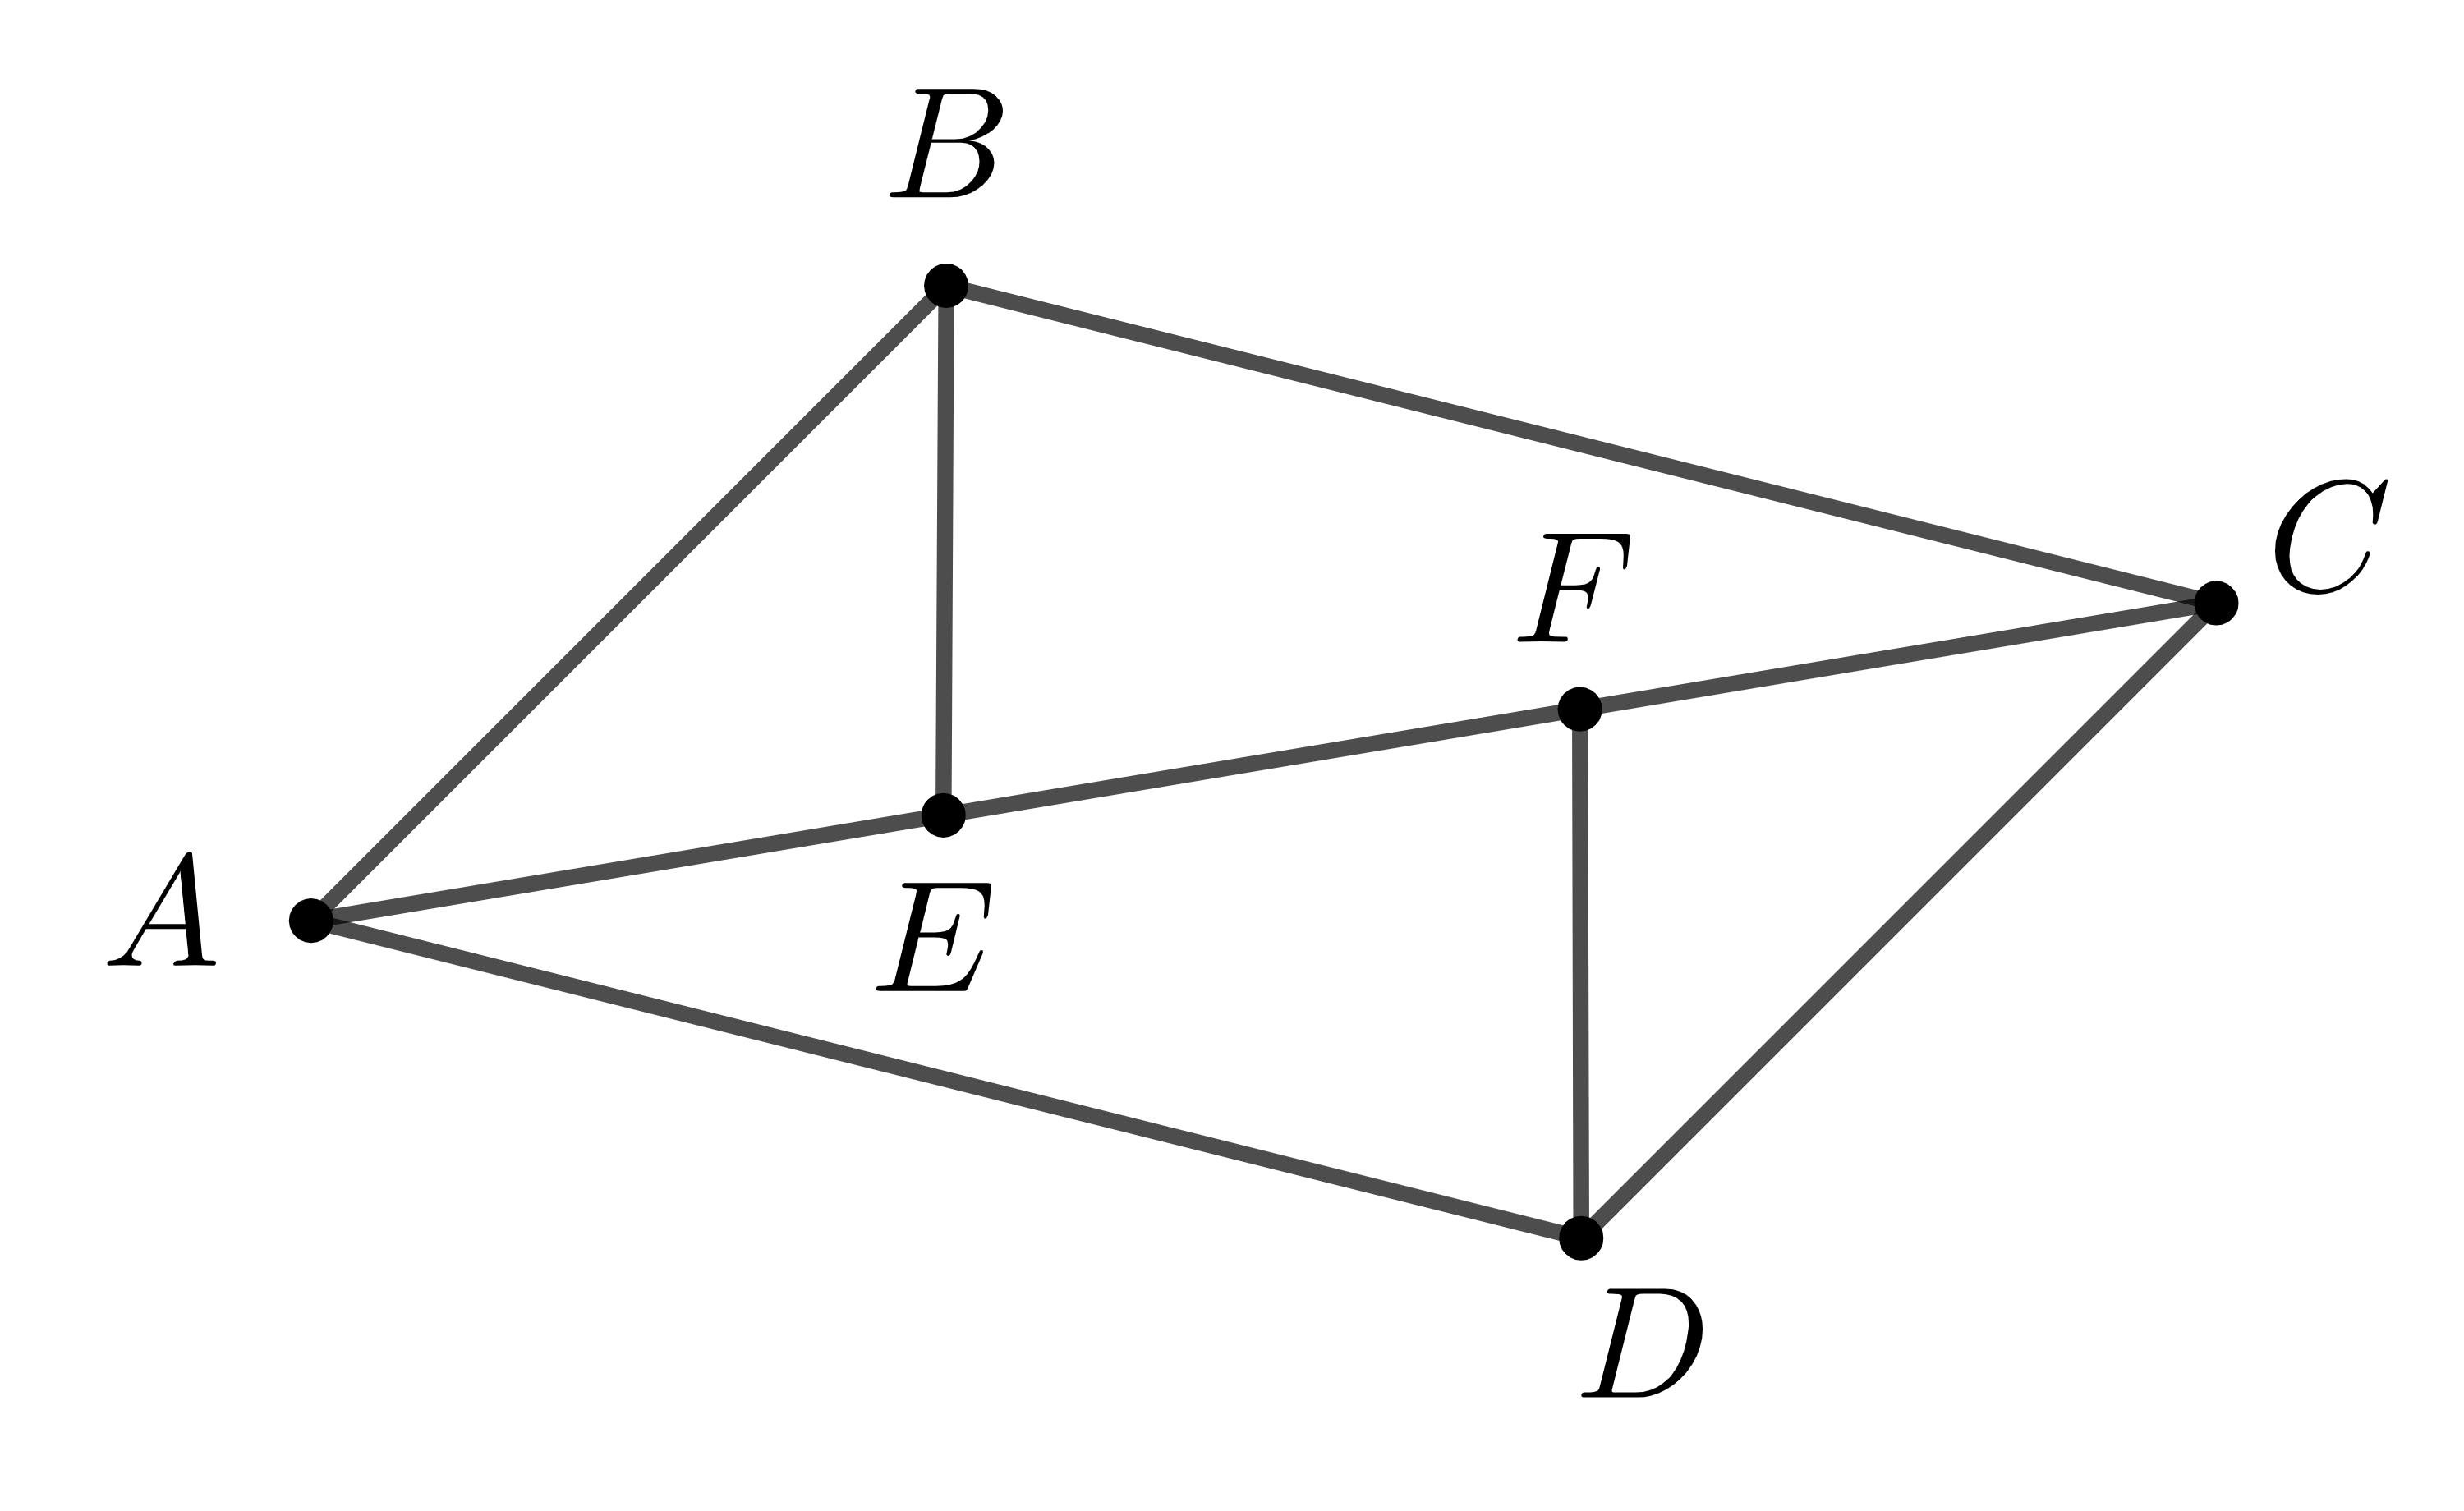
\includegraphics[width=.3\textwidth]{real_exams/7_math_for_8_inzh/pics/202606_inzh_1.png}
\end{problem}

\noindent\grid{34}{18}

\begin{center}
\textbf{Дополнительные задачи}
\end{center}

\samerowans{\begin{problem}{11 (5 баллов)}
Высоты равнобедренного треугольника, проведённые к боковым сторонам, пересекаются под углом $150^{\text{o}}$. Найдите углы треугольника.
\end{problem}}

\smallskip

\samerowans{\begin{problem}{12 (5 баллов)}
Какое число надо прибавить к многочлену $9x^2 - 60x - 2$, чтобы получить квадрат двучлена?
\end{problem}}

\smallskip

\begin{problem}{13 (10 баллов)}
Докажите, что разность квадратов двух последовательных натуральных нечётных чисел равна удвоенной сумме этих чисел.
\end{problem}

\smallskip

\noindent\grid{34}{18}